



\subsection{Agentic Feedback Mechanisms}

Agentic feedback mechanisms enable models to iteratively refine their reasoning and actions rather than relying on one-shot responses. By incorporating self-critique, verifier guidance, or validator-based resampling, these methods emulate human trial-and-error learning and form the foundation for autonomous self-improvement. Broadly, they operate through three distinct feedback regimes:
(1) reflective feedback, where models revise their reasoning through self-critique or verification;
(2) parametric adaptation, where feedback is consolidated into updated model parameters; and
(3) validator-driven feedback, where binary outcome signals guide resampling without introspection.

These regimes define a continuum between dynamic, inference-time adaptability, durable learning through parameter updates, and efficient correction through external signals. Together, they highlight how modern agents leverage feedback to balance flexibility, reliability, and efficiency.

\subsubsection{Reflective Feedback}

Reflective feedback methods improve model reliability by modifying the reasoning process during inference, without updating model parameters. These approaches expose intermediate reasoning outputs, such as chains of thought or partial solutions, and introduce additional assessment steps that directly influence how the model continues its generation.

Early self-critique and rationale-refinement methods \cite{shinn2023reflexion,madaan2023self} implement reflection through an explicit generate–critique–revise loop. A model first produces an answer together with its reasoning. The same model, or a separately prompted critic role, then analyzes this output to identify logical errors, unsupported assumptions, or missing steps. The critique is appended as context for a revised generation, and this process may be repeated multiple times or augmented with external evidence such as retrieval. More recent self-improvement frameworks \cite{selfimprovement2024a} extend reflective feedback beyond a single inference episode by accumulating critiques or failure cases across interactions. Instead of correcting only one response, these methods reuse past feedback to guide future generations through prompt refinement or curated supervision signals, while still operating without direct parameter updates at inference time. Search-based reasoning strategies \cite{wangself,yao2023tree,besta2024graph} improve reliability by generating and comparing multiple candidate reasoning paths. These methods explore the solution space through stochastic sampling or structured search, then select or aggregate outputs using voting schemes, heuristic scores, or learned evaluators. Improvement arises from comparison across alternatives rather than explicit revision of a single reasoning trajectory. Decomposition-based prompting methods \cite{zhou2022least,chenprogram} reformulate complex problems into ordered sequences of simpler subproblems. Intermediate results are reused in later steps, allowing partial inspection of reasoning progress and reducing error propagation, even when no explicit critique step is introduced.

Overall, reflective feedback alters inference-time reasoning trajectories by introducing additional reasoning or comparison steps. Feedback is used to guide generation within an episode, while the model’s parameters remain unchanged.

\begin{figure}
    \centering
    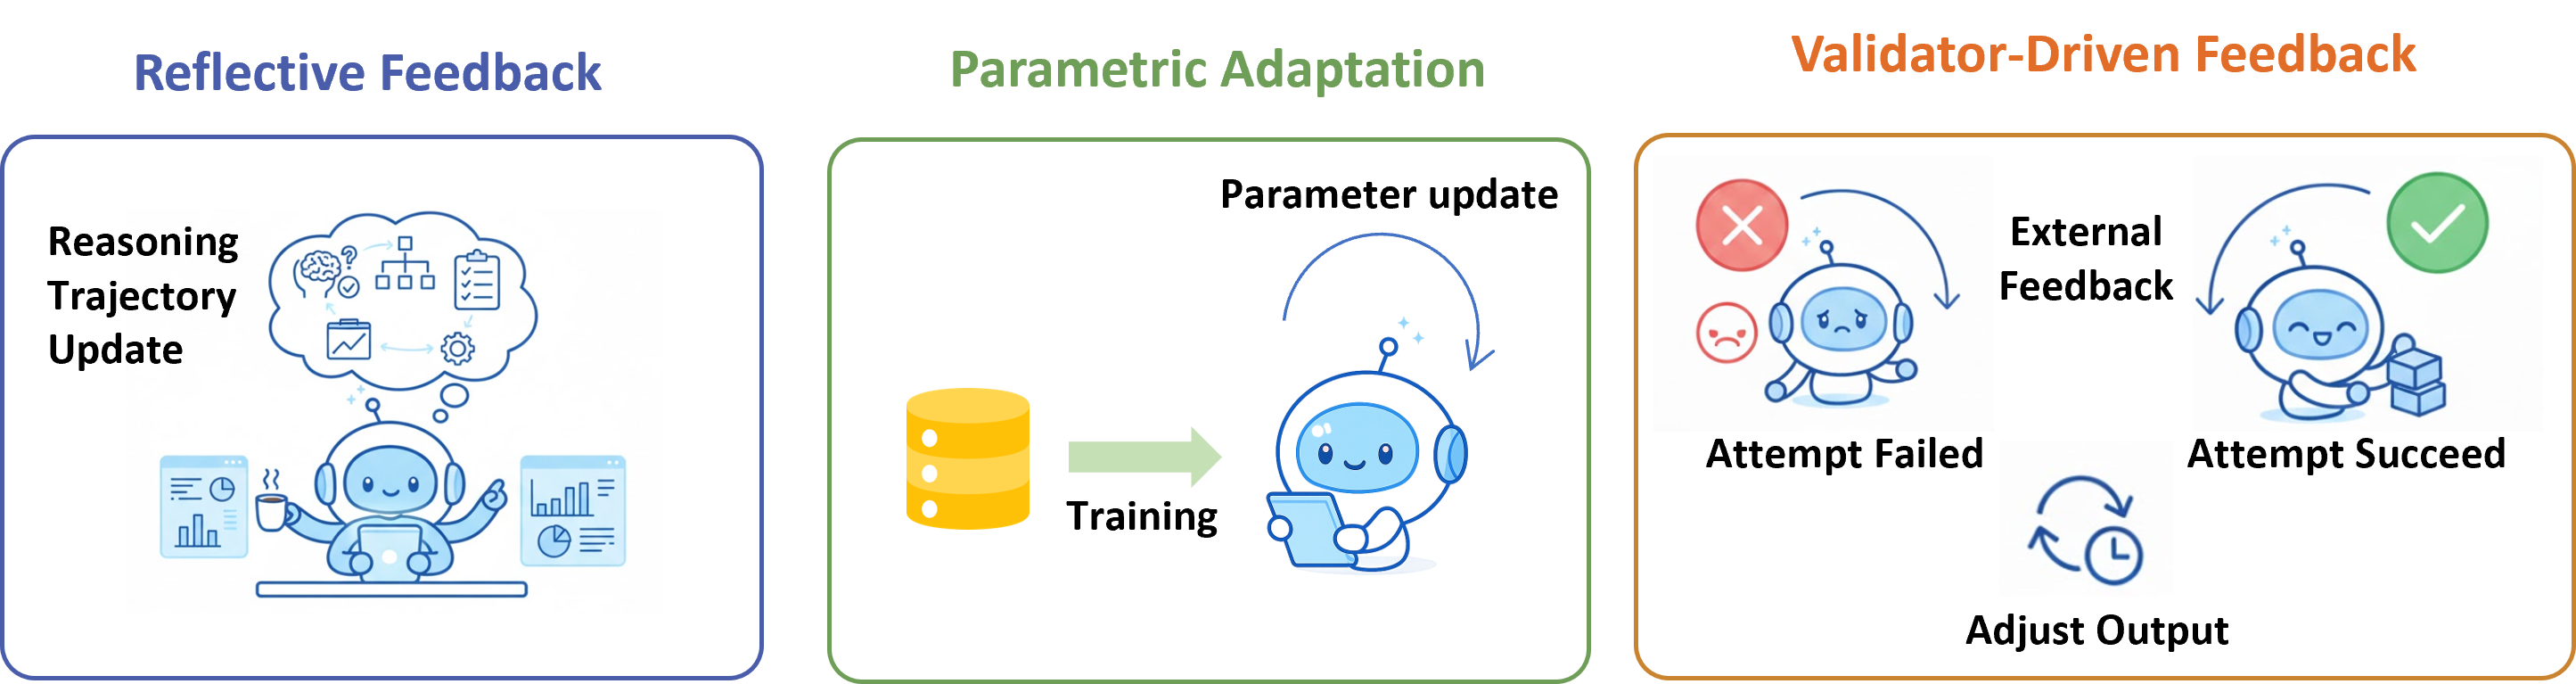
\includegraphics[width=\linewidth]{arxiv/figs/feedback.png}
    \caption{
    \textbf{Illustration of three forms of agentic feedback mechanisms.}
    \textit{Inference-time reflection} enables real-time self-critique and revision during reasoning;
    \textit{offline adaptation} consolidates feedback into model parameters for long-term improvement;
    and \textit{outcome-based feedback} relies on validator signals (success or failure) to refine behavior through retry.
    Together, they represent a continuum from adaptive reflection to stable learning and efficient validation.
    }
    \label{fig:agentic_feedback}
\end{figure}

\subsubsection{Parametric Adaptation}

Parametric adaptation incorporates feedback into a model’s parameters through additional training, producing persistent behavioral changes that generalize beyond individual inference episodes. Unlike reflective feedback, these methods transform feedback signals into supervised or preference-based training objectives that update the model’s weights.

Trajectory-level supervised fine-tuning approaches \cite{zeng2024agenttuning,aksitov2023rest} attach feedback to intermediate reasoning traces rather than only final answers. Models first generate multi-step trajectories, which are then reviewed by humans, auxiliary models, or automated verifiers. Incorrect steps are corrected or replaced, and the resulting feedback-enriched trajectories are used as supervised training data, encouraging the model to internalize improved reasoning patterns. Distillation-based methods \cite{hsieh2023distilling} further leverage improved reasoning traces by training student models on high-quality chains of thought or self-corrected solutions generated by stronger teachers. This process transfers structured reasoning behaviors into more stable or efficient models, removing the need for explicit reflection at inference time. Preference-alignment approaches \cite{christiano2017deep,rafailov2023dpo,bai2022constitutional} incorporate feedback in the form of comparative judgments that distinguish preferred from dispreferred outputs. Training objectives such as reward modeling or direct preference optimization adjust the model’s parameters so that preferred behaviors become more likely. Although feedback is often defined over final outputs, it implicitly shapes the internal reasoning strategies that produce them. Recent work shows that verification-augmented training data can further improve reasoning robustness across domains \cite{li2025reflectevo,zheng2025reasoningcv}. In these settings, trajectories are filtered or revised based on correctness or consistency signals before training, yielding datasets that emphasize reliable reasoning patterns.

In summary, parametric adaptation embeds feedback directly into the model’s parameters, yielding durable improvements across tasks. This durability comes at the cost of additional training and reduced flexibility compared to inference-time methods.

\subsubsection{Validator-Driven Feedback}

Validator-driven feedback improves model outputs using external success or failure signals, without modifying the model’s reasoning process or parameters. A validator, such as a unit test, constraint checker, simulator, or environment signal, evaluates candidate outputs and determines whether they satisfy predefined correctness criteria.

Retry-based systems \cite{dao2025rezero,potamitis2025retrials} implement this paradigm by repeatedly sampling candidate outputs until one passes validation. The model generates a complete solution, submits it to the validator, and discards it if validation fails. Subsequent attempts are generated independently, without conditioning on explicit information about previous failures. This strategy is particularly effective in domains with reliable and inexpensive validation, such as program synthesis and software engineering \cite{le2022coderl,ni2023lever,swebench}. Generated code can be executed against unit tests, providing an unambiguous correctness signal. The model iterates until a solution satisfies all tests, even in the absence of explicit reasoning correction. Similar mechanisms appear in embodied and interactive agents \cite{ahn2022icanisay,driess2023palm}, where action sequences are repeatedly executed until the environment signals task completion. Failed sequences are abandoned and new ones are attempted, based solely on external success signals. Some hybrid methods introduce lightweight guidance within the retry loop, for example by assigning higher reward to behaviors that eventually lead to successful outcomes \cite{bensal2025reflect}. However, the dominant mechanism remains selection through external validation rather than revision of reasoning steps or parameter updates.

Overall, validator-driven feedback offers an efficient and scalable way to improve output correctness when reliable validators are available. Its limitation is that feedback is non-diagnostic, correcting individual outputs without explaining failures or altering the model’s reasoning behavior.

\begin{table*}[!t]
\centering
\caption{Representative \textbf{Agentic Feedback Mechanisms} categorized by \textit{Feedback Stage}, \textit{Feedback Source}, and \textit{Update Target}.}
\renewcommand{\arraystretch}{1.15}
\setlength{\tabcolsep}{3pt}
\begin{tabular}{p{5.5cm}
  >{\centering\arraybackslash}p{3.8cm}
  >{\centering\arraybackslash}p{4.8cm}
  >{\centering\arraybackslash}p{3.3cm}}
\toprule
\textbf{Method / System} & \textbf{Feedback Stage} & \textbf{Feedback Source} & \textbf{Update Target} \\
\midrule

%%%%%%%%%%%%%%%%%%%%%%%%%%%%%%%%%%%%%%%%%%%%%%%%%%%%%%%%%%%%%%
% I. Reflective Feedback
%%%%%%%%%%%%%%%%%%%%%%%%%%%%%%%%%%%%%%%%%%%%%%%%%%%%%%%%%%%%%%
\rowcolor[HTML]{F5F5F5}
\multicolumn{4}{l}{\textbf{I. Reflective Feedback}} \\

Reflexion~\cite{shinn2023reflexion} & Inference & Self-generated critique & Trajectory \\
Self-Refine~\cite{madaan2023self} & Inference & Self-evaluation & Trajectory \\
Constitutional AI~\cite{bai2022constitutional} & Inference & Normative rules & Trajectory \\
RLAIF~\cite{lee2023rlaif} & Inference & AI verifier & Trajectory \\
SelfCheckGPT~\cite{manakul2023selfcheckgpt} & Inference & Cross-sample divergence & Trajectory \\
Zero-Shot Verification-CoT~\cite{chowdhury2025zeroshot} & Inference & External verifier & Trajectory \\
ASCoT~\cite{zhang2025ascot} & Inference & Vulnerability detection & Trajectory \\
MM-Verify~\cite{sun2025mmverify} & Inference & Multimodal verifier & Trajectory \\
ReAct~\cite{yao2023react} & Inference & Action outcomes & Trajectory \\
PAL~\cite{gao2023pal} & Inference & Code execution & Trajectory \\
WebGPT~\cite{nakano2021webgpt} & Inference & Web evidence & Trajectory \\
MemGPT~\cite{Packer2023MemGPTTL} & Inference & Retrieved memory & Trajectory \\
Voyager~\cite{wang2023voyager} & Inference & Environment + memory & Trajectory \\

\midrule

%%%%%%%%%%%%%%%%%%%%%%%%%%%%%%%%%%%%%%%%%%%%%%%%%%%%%%%%%%%%%%
% II. Parametric Adaptation
%%%%%%%%%%%%%%%%%%%%%%%%%%%%%%%%%%%%%%%%%%%%%%%%%%%%%%%%%%%%%%
\rowcolor[HTML]{F5F5F5}
\multicolumn{4}{l}{\textbf{II. Parametric Adaptation}} \\

AgentTuning~\cite{zeng2024agenttuning} & Training & High-quality trajectories & Model parameters \\
ReST~\cite{aksitov2023rest} & Training & Critique--revision pairs & Model parameters \\
ReFT~\cite{dou2024re} & Training & Reflection-augmented data & Model parameters \\
Distill-CoT~\cite{hsieh2023distilling} & Training & Expert CoT & Model parameters \\
ReflectEvo~\cite{li2025reflectevo} & Training & Reflection traces & Model parameters \\
Reasoning-CV~\cite{zheng2025reasoningcv} & Training & Verification signals & Model parameters \\

\midrule

%%%%%%%%%%%%%%%%%%%%%%%%%%%%%%%%%%%%%%%%%%%%%%%%%%%%%%%%%%%%%%
% III. Validator-Driven Feedback
%%%%%%%%%%%%%%%%%%%%%%%%%%%%%%%%%%%%%%%%%%%%%%%%%%%%%%%%%%%%%%
\rowcolor[HTML]{F5F5F5}
\multicolumn{4}{l}{\textbf{III. Validator-Driven Feedback}} \\

ReZero~\cite{dao2025rezero} & Inference & Binary validator & Output only \\
Retrials~\cite{potamitis2025retrials} & Inference & Acceptance signal & Output only \\
CodeRL~\cite{le2022coderl} & Inference & Unit tests & Output only \\
LEVER~\cite{ni2023lever} & Inference & Execution results & Output only \\
SWE-bench~\cite{swebench} & Inference & Test suite & Output only \\
SayCan~\cite{ahn2022icanisay} & Inference & Environment state & Output only \\
PaLM-E~\cite{driess2023palm} & Inference & Environment feedback & Output only \\
Reflect--Retry--Reward~\cite{bensal2025reflect} & Inference & Validator + reflection signal & Output only \\

\bottomrule
\end{tabular}
\label{tab:agentic_feedback_methods}
\end{table*}

